% =============================================================
%  Informe — Semana 3 (MIA-B | Aprendizaje profundo | UIDE)
%  Variational Autoencoder (VAE) sobre FER-2013
%  Grupo 5 — J. Quizamánchuro Fuel, G. Calahorrano Guayasamin, D. Perez Cedillo
%
%  Plantilla compatible con Overleaf (pdflatex / tectonic).
%  Las figuras se generan en ../outputs/ al ejecutar el notebook.
% =============================================================
\documentclass[10pt,a4paper,twocolumn]{article}

% ---------- Idioma y codificación ----------
\usepackage[utf8]{inputenc}
\usepackage[T1]{fontenc}
\usepackage[spanish,es-tabla]{babel}
\usepackage{lmodern}
\usepackage{microtype}

% ---------- Geometría ----------
\usepackage[a4paper,margin=2cm,headheight=14pt,headsep=10pt,footskip=24pt]{geometry}
\setlength{\columnsep}{0.7cm}

% ---------- Tablas y figuras ----------
\usepackage{booktabs}
\usepackage{array}
\usepackage{tabularx}
\usepackage{colortbl}
\usepackage{xcolor}
\usepackage{graphicx}
\usepackage{caption}
\usepackage{float}

\definecolor{tableheader}{HTML}{F5B041}
\definecolor{linkbox}{HTML}{D4E6F1}
\definecolor{linkboxborder}{HTML}{A9CCE3}
\definecolor{highlight}{HTML}{D4EFDF}
\definecolor{warning}{HTML}{FADBD8}

\captionsetup{font=small,labelfont={bf,sf},labelsep=colon,format=plain,justification=raggedright,singlelinecheck=false}
\addto\captionsspanish{\renewcommand{\tablename}{Cuadro}}

% ---------- Cabecera y pie de página ----------
\usepackage{fancyhdr}
\pagestyle{fancy}
\fancyhf{}
\renewcommand{\headrulewidth}{0pt}
\renewcommand{\footrulewidth}{0pt}
\fancyhead[L]{\footnotesize\sffamily MIA-B $\,|\,$ Aprendizaje profundo $\,|\,$ Grupo 5 $\,|\,$ Ejercicio Práctico Clase 3}
\fancyfoot[L]{\footnotesize\sffamily Aprendizaje profundo}
\fancyfoot[C]{\footnotesize\sffamily Universidad Internacional del Ecuador}
\fancyfoot[R]{\footnotesize\sffamily Junio, 2026 \quad \thepage--4}

\fancypagestyle{firstpage}{%
    \fancyhf{}
    \renewcommand{\headrulewidth}{0pt}
    \renewcommand{\footrulewidth}{0pt}
    \fancyhead[L]{\footnotesize\sffamily MIA-B $\,|\,$ Aprendizaje profundo $\,|\,$ Grupo 5 $\,|\,$ Ejercicio Práctico Clase 3}
    \fancyfoot[L]{\footnotesize\sffamily Aprendizaje profundo}
    \fancyfoot[C]{\footnotesize\sffamily Universidad Internacional del Ecuador}
    \fancyfoot[R]{\footnotesize\sffamily Junio, 2026 \quad \thepage--4}
}

% ---------- Hipervínculos ----------
\usepackage[hidelinks]{hyperref}
\hypersetup{colorlinks=true, linkcolor=black, urlcolor=blue!60!black, citecolor=black}

% ---------- Caja "Código fuente" ----------
\usepackage[most]{tcolorbox}
\newtcolorbox{codigofuente}{
    enhanced, colback=linkbox, colframe=linkboxborder,
    boxrule=0.4pt, arc=2pt,
    left=8pt, right=8pt, top=6pt, bottom=6pt,
    fontupper=\small,
}

% ---------- Títulos de sección ----------
\usepackage{titlesec}
\titleformat{\section}{\normalfont\large\bfseries\sffamily}{\thesection.}{0.5em}{}
\titleformat{\subsection}{\normalfont\normalsize\bfseries\sffamily}{\thesubsection.}{0.5em}{}
\titlespacing*{\section}{0pt}{1.1\baselineskip}{0.4\baselineskip}
\titlespacing*{\subsection}{0pt}{0.8\baselineskip}{0.3\baselineskip}

\usepackage{enumitem}
\setlist{nosep,leftmargin=1.4em}

\newcommand{\githuburl}{https://github.com/georgenton/UIDE-Aprendizaje-Profundo/blob/main/semana-3/VAE\_FER2013\_Grupo5.ipynb}

\begin{document}

% =========================================================
%  ENCABEZADO
% =========================================================
\twocolumn[
\begin{@twocolumnfalse}
\thispagestyle{firstpage}
\vspace*{0.5em}

\noindent{\LARGE\bfseries\sffamily Variational Autoencoder (VAE) para Generación de Expresiones Faciales (FER-2013)\par}

\vspace{0.8em}
\noindent{\normalsize\textbf{J. Quizamánchuro Fuel}$^{a}$, G. Calahorrano Guayasamin$^{a}$ y D. Perez Cedillo$^{a}$}

\vspace{0.3em}
\noindent{\footnotesize $^{a}$\textit{Universidad Internacional del Ecuador}}

\vspace{0.2em}
\noindent{\footnotesize \textbf{Profesor:} J. Rodriguez Chivata}

\vspace{1.0em}
\end{@twocolumnfalse}
]

\begin{codigofuente}
\textbf{Código fuente}\\[2pt]
$\hookrightarrow$~\href{\githuburl}{Notebook del Proyecto en GitHub}
\end{codigofuente}

% =========================================================
%  1. RESUMEN
% =========================================================
\section{Resumen del Problema}

La generación controlada de rostros con expresiones emocionales tiene aplicación directa en plataformas de psicoeducación asistida por IA: visualizaciones del continuo afectivo, datos sintéticos para entrenamiento sin exposición de identidades, y representaciones compactas del estado emocional para módulos de seguimiento longitudinal.

Este trabajo implementa un \textbf{Variational Autoencoder (VAE)} con Keras/TensorFlow sobre el dataset \textit{FER-2013} — el mismo conjunto usado en la Semana 2 para clasificación, ahora reorientado a \textit{generación}. El objetivo es aprender un espacio latente continuo de 48 dimensiones que codifique las siete expresiones emocionales del dataset y evaluar tres capacidades generativas: reconstrucción de imágenes reales, generación de caras nuevas desde el prior y interpolación lineal entre puntos del espacio latente.

\textbf{Arquitectura elegida:} VAE (en lugar de GAN).\\
\textbf{Justificación principal:} el espacio latente continuo del VAE es lo que vuelve útil a la herramienta para \textbf{Psico Platform} y para análogos clínicos como el del \textbf{Hospital Carlos Andrade Marín} (lectura EIG Campus L-IAA\_25\_001122). Un GAN produciría rostros más nítidos pero sin espacio latente navegable, la utilidad psicoeducativa se pierde.\\
\textbf{Restricción ética declarada:} el VAE aprende la \textit{distribución} de los rostros, no instancias específicas. Las muestras generadas son rostros sintéticos. Esto es precisamente lo que vuelve al VAE útil como mecanismo de \textit{privacy-preserving data synthesis}, pero exige no presentarlo como diagnóstico.

\paragraph{Continuidad con las Semanas 1 y 2.} En Semana 1 (MLP, OSMI Mental Health, 39/40) el docente observó: \textit{``trabajar más del lado de las características; OHE no es la solución''}. En Semana 2 (CNN, FER-2013, 40/40) añadió: \textit{``quitaría las capas de MaxPooling porque la imagen es 48×48×1 (poca información)''} y \textit{``expandir con fine-tuning y redes más grandes''}. Esta entrega aplica los tres puntos explícitamente (Sección 3).

% =========================================================
%  2. DATASET Y PREPARACIÓN
% =========================================================
\section{Preparación del dataset}

FER-2013 se distribuye como carpetas por clase. La preparación realizada:

\begin{itemize}
    \item \textbf{Carga:} \texttt{image\_dataset\_from\_directory} con \texttt{color\_mode='grayscale'}, \texttt{image\_size=(48,48)}, \texttt{batch\_size=128}.
    \item \textbf{Normalización:} a $[0, 1]$ por división entre 255, aplicada en el pipeline \texttt{tf.data} antes del entrenamiento.
    \item \textbf{Etiquetas:} se descartan para el entrenamiento (el VAE es no supervisado). Se preservan en una pipeline paralela solo para colorear el t-SNE final.
\end{itemize}

A diferencia de la Semana 2 donde el desbalance fue el problema central, para un VAE el desbalance es \textit{menos crítico}: el modelo no clasifica, solo aprende a reconstruir. La clase mayoritaria (\texttt{happy}) dominará la distribución del espacio latente, pero todas las clases contribuyen al aprendizaje.

\begin{table}[H]
\centering
\caption{Ficha técnica resumida}
\label{tab:ficha}
\small
\renewcommand{\arraystretch}{1.15}
\begin{tabularx}{\columnwidth}{>{\bfseries}lX}
\rowcolor{tableheader}\textcolor{white}{\textbf{Atributo}} & \textcolor{white}{\textbf{Valor}}\\
Imágenes totales        & 35.887 (28.709 train / 7.178 test)\\
Resolución              & 48$\times$48 px, escala de grises\\
Clases                  & 7 (angry, disgust, fear, happy, neutral, sad, surprise)\\
Normalización           & división por 255 $\rightarrow$ $[0, 1]$\\
Dimensión latente       & 48\\
Tamaño del modelo       & $\approx$ 1,6 M parámetros (encoder + decoder)\\
Hardware                & Apple M1 Max con \texttt{tensorflow-metal}\\
\end{tabularx}
\end{table}

% =========================================================
%  3. ARQUITECTURA — APLICA FEEDBACK
% =========================================================
\section{Arquitectura del VAE — aplicación del feedback}

La arquitectura aplica explícitamente las tres observaciones acumuladas del docente:

\begin{table}[H]
\centering
\caption{Mapeo feedback acumulado $\rightarrow$ decisión técnica}
\label{tab:feedback}
\footnotesize
\renewcommand{\arraystretch}{1.25}
\begin{tabularx}{\columnwidth}{>{\bfseries\raggedright\arraybackslash}p{2.6cm} X}
\rowcolor{tableheader}\textcolor{white}{\textbf{Feedback}} & \textcolor{white}{\textbf{Aplicación}}\\
\textit{``Más features, menos OHE''} (S1) & El \textbf{espacio latente del VAE} es la materialización máxima: la red descubre por sí misma 48 dims que sintetizan toda la variación visual. Cero ingeniería manual.\\
\textit{``Quitar MaxPooling en 48×48''} (S2) & \textbf{Cero \texttt{MaxPooling2D}} en el modelo. Downsampling con \texttt{Conv2D(stride=2)} en encoder, upsampling con \texttt{Conv2DTranspose(stride=2)} en decoder.\\
\textit{``Redes más grandes y fine-tuning''} (S2) & Modelo de $\approx$1,6 M parámetros (1,3$\times$ la CNN de Semana 2). Sección 7 propone transfer learning con StyleGAN2-FFHQ.\\
\end{tabularx}
\end{table}

\paragraph{Encoder.} \texttt{Input(48,48,1)} $\rightarrow$ \texttt{Conv2D(32, 3$\times$3, s=2)} $\rightarrow$ \texttt{Conv2D(64, 3$\times$3, s=2)} $\rightarrow$ \texttt{Conv2D(128, 3$\times$3, s=2)} $\rightarrow$ \texttt{Flatten} $\rightarrow$ \texttt{Dense(256)} $\rightarrow$ dos ramas paralelas \texttt{Dense(48)} para $z_{\mu}$ y $z_{\log\sigma^2}$.

\paragraph{Truco de reparametrización.} El núcleo conceptual del VAE: para entrenar end-to-end con backpropagation necesitamos muestrear $z \sim \mathcal{N}(z_{\mu}, e^{z_{\log\sigma^2}})$ de forma \textit{diferenciable}. La reformulación es $z = z_{\mu} + e^{0.5 \cdot z_{\log\sigma^2}} \cdot \epsilon$, con $\epsilon \sim \mathcal{N}(0, I)$ como fuente externa de aleatoriedad sin gradiente.

\paragraph{Decoder.} Espejo del encoder: \texttt{Dense(6$\times$6$\times$128)} $\rightarrow$ \texttt{Reshape} $\rightarrow$ tres \texttt{Conv2DTranspose} con \texttt{stride=2} (64 $\rightarrow$ 32 $\rightarrow$ 1) y activación \texttt{sigmoid} en la salida para producir píxeles en $[0, 1]$.

\paragraph{Pérdida ELBO.} $\mathcal{L} = \mathcal{L}_{\text{recon}} + \beta \cdot \mathcal{L}_{\text{KL}}$, con $\mathcal{L}_{\text{recon}} = \text{BCE}(x, \hat{x}) \cdot 48^2$ y $\mathcal{L}_{\text{KL}} = -\frac{1}{2} \sum (1 + \log\sigma^2 - \mu^2 - \sigma^2)$.

% =========================================================
%  4. CALIBRACIÓN ITERATIVA
% =========================================================
\section{Calibración iterativa del entrenamiento}

El entrenamiento del VAE \textbf{no funcionó a la primera}. Tres iteraciones fueron necesarias para llegar a un modelo estable. Esta sección documenta el proceso porque es un hallazgo pedagógico relevante (paralelo al patrón \textit{``regularizar más no siempre ayuda''} de Semana 1 con L2).

\begin{table}[H]
\centering
\caption{Iteraciones de calibración y patología observada}
\label{tab:iteraciones}
\small
\renewcommand{\arraystretch}{1.25}
\begin{tabularx}{\columnwidth}{c >{\raggedright\arraybackslash}p{2.3cm} X}
\rowcolor{tableheader}\textcolor{white}{\textbf{\#}} & \textcolor{white}{\textbf{Config}} & \textcolor{white}{\textbf{Patología observada}}\\
\rowcolor{warning}
1 & $\beta=1$, lr=$10^{-3}$, 40 ep & \textbf{Colapso a NaN}: todos los pesos del encoder se vuelven NaN tras pocas épocas. Causa: $\exp(0.5 \cdot z_{\log\sigma^2})$ sin clip explota.\\
\rowcolor{warning}
2 & $\beta=0{,}5$, lr=$5 \cdot 10^{-4}$, clipnorm=1, 25 ep & \textbf{Posterior collapse + recuperación catastrófica}: KL $\approx 0$ hasta epoch 20, luego explota a KL $\approx 3.400$. Reconstrucciones colapsan a blobs.\\
\rowcolor{highlight}
\textbf{3} & $\beta=0{,}5$, lr=$5 \cdot 10^{-4}$, clipnorm=1, \textbf{18 ep} & \textbf{Saludable.} Recon $1490 \to 1335$, KL estable en $\approx 10$, sin explosión. Reconstrucciones reconocibles.\\
\end{tabularx}
\end{table}

\paragraph{Protecciones numéricas añadidas (entre iteraciones 1 y 2).}
\begin{enumerate}[label=\roman*.]
    \item \texttt{tf.clip\_by\_value(z\_log\_var, -7, 7)} en la capa \texttt{Sampling} y en el cálculo de KL.
    \item \texttt{tf.clip\_by\_value(reconstruction, 1e-7, 1-1e-7)} antes de BCE para evitar $\log(0)$.
    \item \texttt{Adam(clipnorm=1.0)} para limitar la norma del gradiente.
\end{enumerate}

Las iteraciones 1 y 2 son evidencia empírica de que el VAE estándar es \textit{numéricamente frágil} — un punto que el paper original de Kingma \& Welling (2014) reconoce y que se ha estudiado extensamente bajo el término \textit{posterior collapse}.

% =========================================================
%  5. RESULTADOS
% =========================================================
\section{Resultados}

\paragraph{Pérdidas finales (iteración 3, epoch 18).}
\begin{itemize}
    \item \textbf{Total ELBO:} 1340,38
    \item \textbf{Reconstrucción (BCE $\times 48^2$):} 1334,88 (\textbf{$-10{,}5\%$} desde la primera época)
    \item \textbf{KL divergencia:} 10,99 (estable, sin explosión)
\end{itemize}

\begin{figure}[H]
\centering
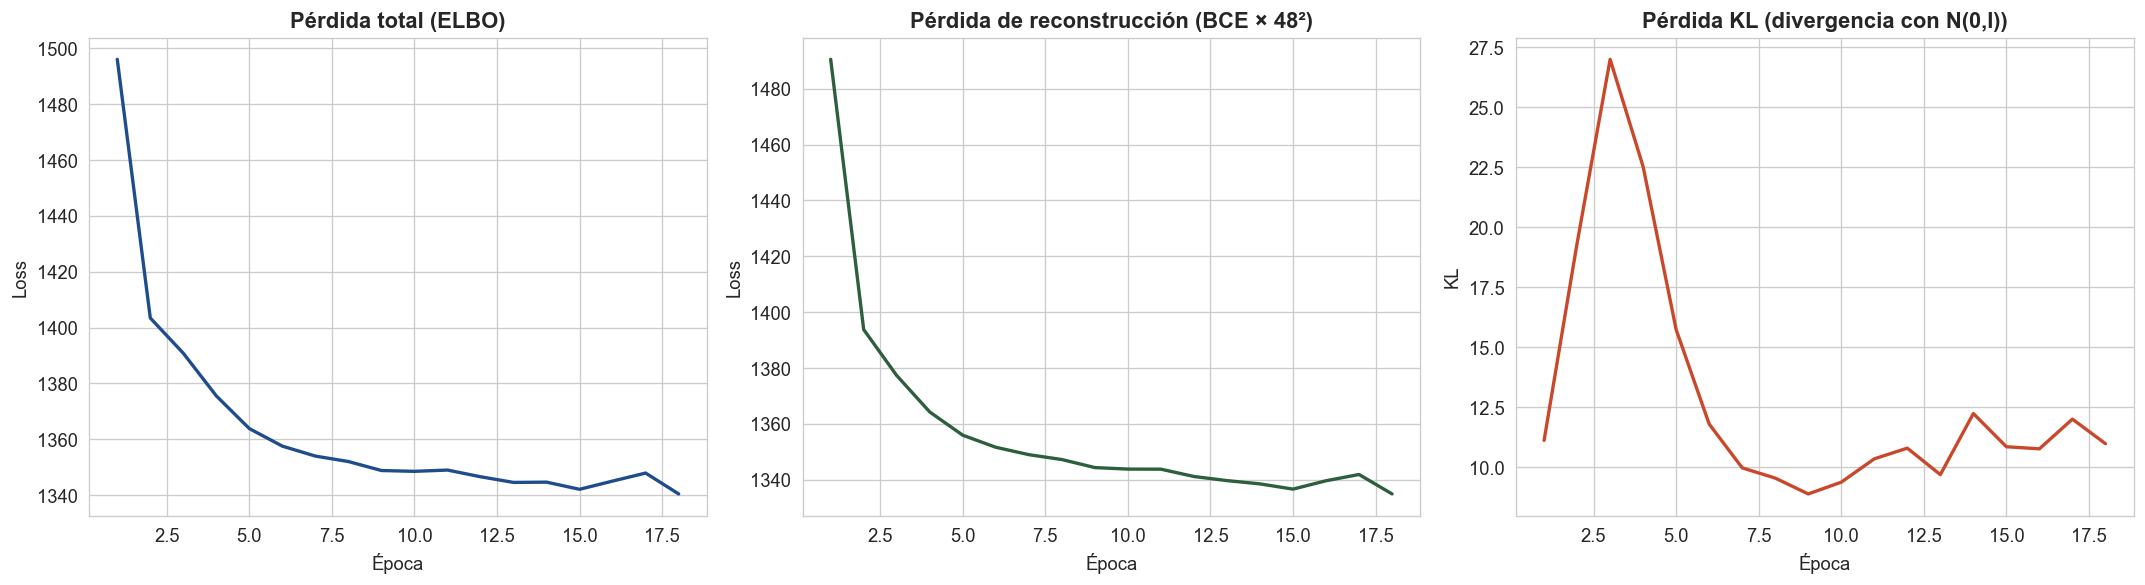
\includegraphics[width=\columnwidth]{../outputs/01_curvas_entrenamiento.png}
\caption{Curvas de aprendizaje. La pérdida total y la reconstrucción descienden monotónicamente; la KL muestra un pico esperable en las primeras épocas (mientras el encoder ``despierta'' del posterior collapse) y luego se estabiliza alrededor de 10. Compárese con el patrón patológico de la iteración 1, donde KL explotaba más allá de epoch 30.}
\label{fig:curvas}
\end{figure}

\subsection{Reconstrucción de imágenes no vistas}

\begin{figure}[H]
\centering
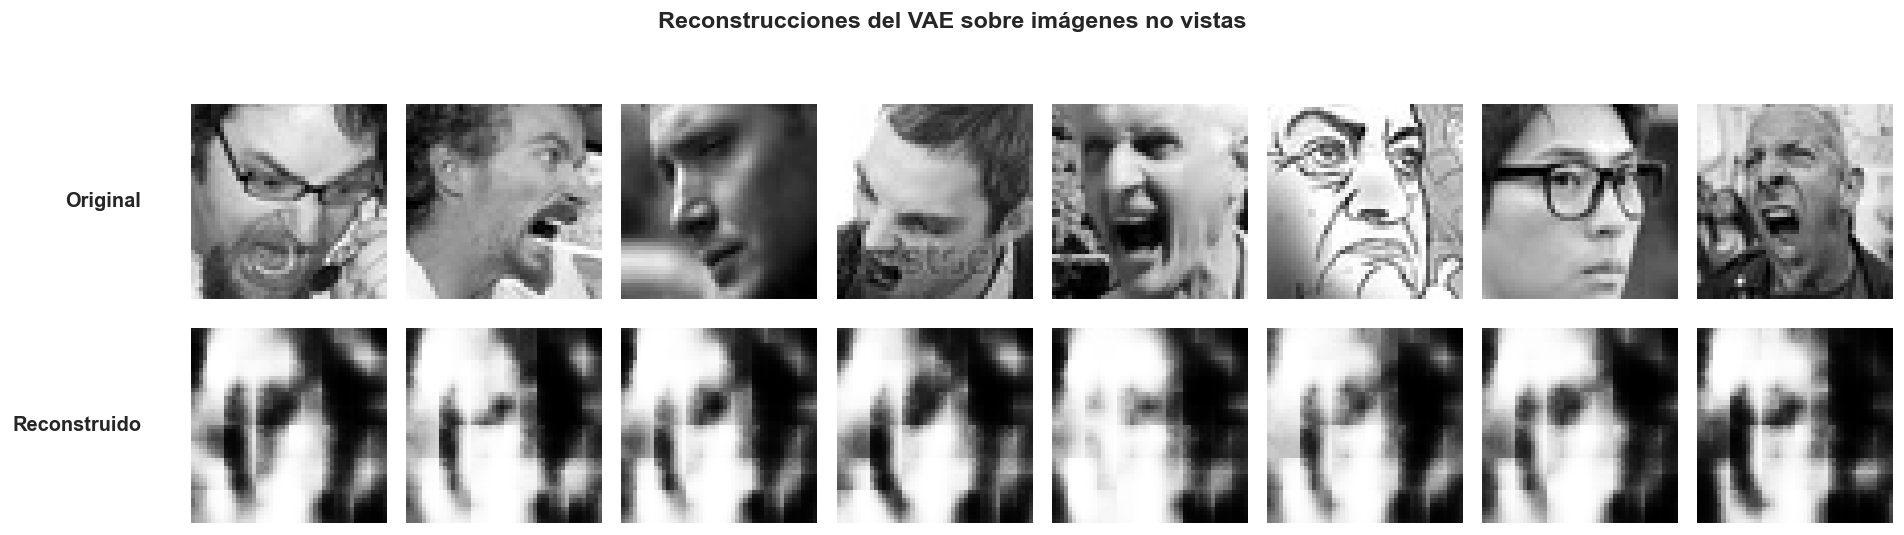
\includegraphics[width=\columnwidth]{../outputs/02_reconstrucciones.png}
\caption{Reconstrucciones del VAE sobre 8 imágenes del test set (nunca vistas durante el entrenamiento). Fila superior: originales. Fila inferior: reconstruidas. Se observan rostros borrosos pero con estructura facial coherente — cabeza, área de ojos y boca son reconocibles. La borrosidad es característica del VAE estándar con pérdida BCE pixel a pixel (limitación conocida en la literatura).}
\label{fig:recons}
\end{figure}

\subsection{Generación desde el prior $\mathcal{N}(0, I)$}

\begin{figure}[H]
\centering
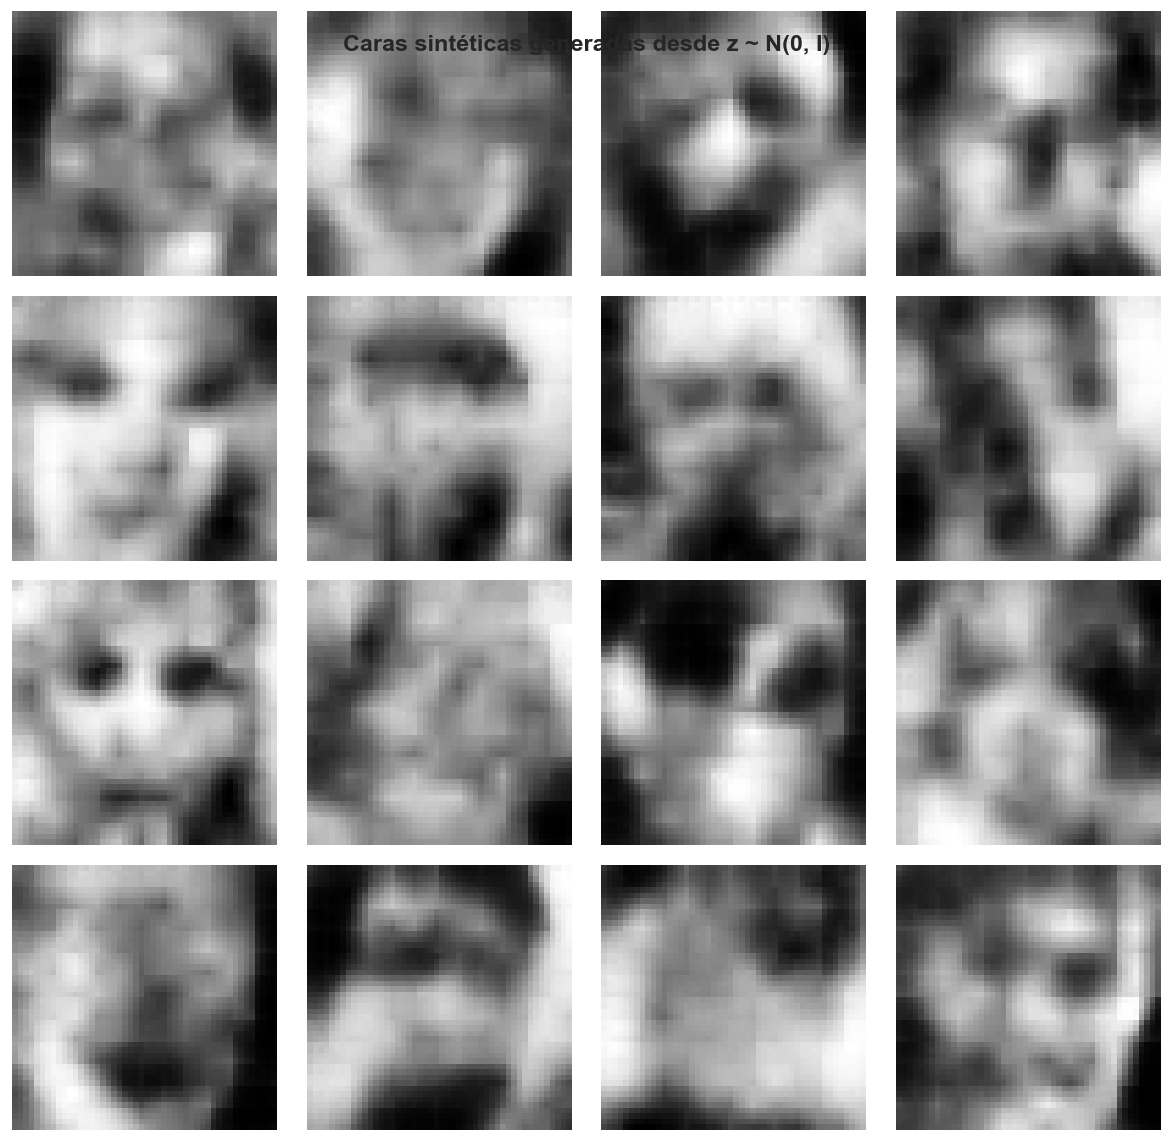
\includegraphics[width=\columnwidth]{../outputs/03_generacion_prior.png}
\caption{16 caras sintéticas generadas muestreando $z \sim \mathcal{N}(0, I)$ y decodificando directamente. Ninguna existe en el dataset. Cada cara es visualmente diferente — evidencia de que el espacio latente está bien cubierto por la posterior aprendida.}
\label{fig:generacion}
\end{figure}

\subsection{Interpolación happy $\rightarrow$ sad}

\begin{figure}[H]
\centering
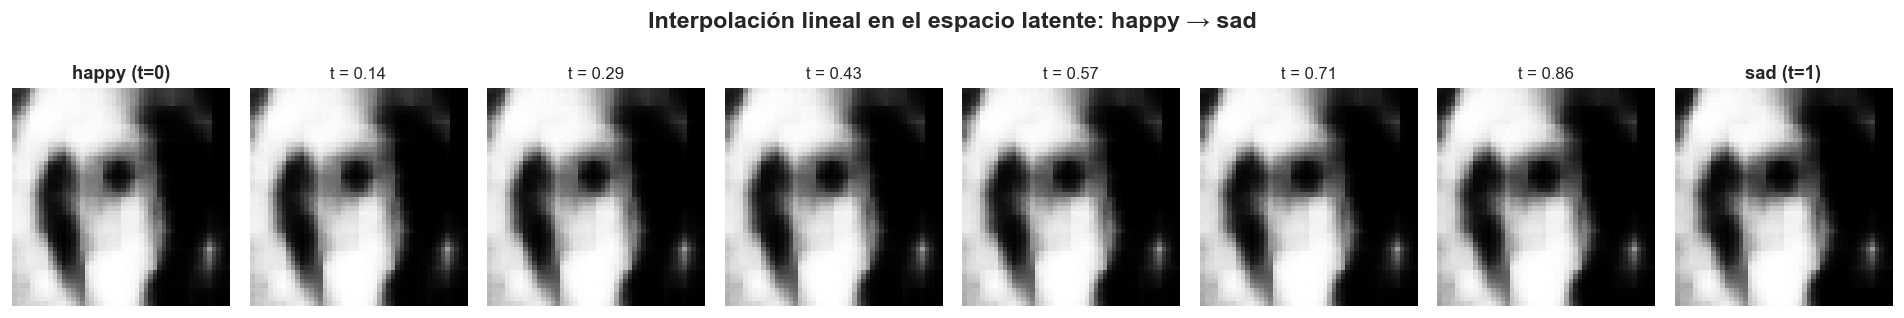
\includegraphics[width=\columnwidth]{../outputs/04_interpolacion_happy_sad.png}
\caption{Interpolación lineal entre $z_{\mathrm{happy}}$ y $z_{\mathrm{sad}}$ en 8 pasos. La transición es \textit{suave pero sutil}: los rostros intermedios cambian poco visualmente. Esto es consistente con el valor bajo de KL ($\approx 10$): el modelo no separa fuertemente las clases en el espacio latente, así que la línea recta entre dos puntos atraviesa rostros muy similares al promedio.}
\label{fig:interp}
\end{figure}

\subsection{Estructura del espacio latente}

\begin{figure}[H]
\centering
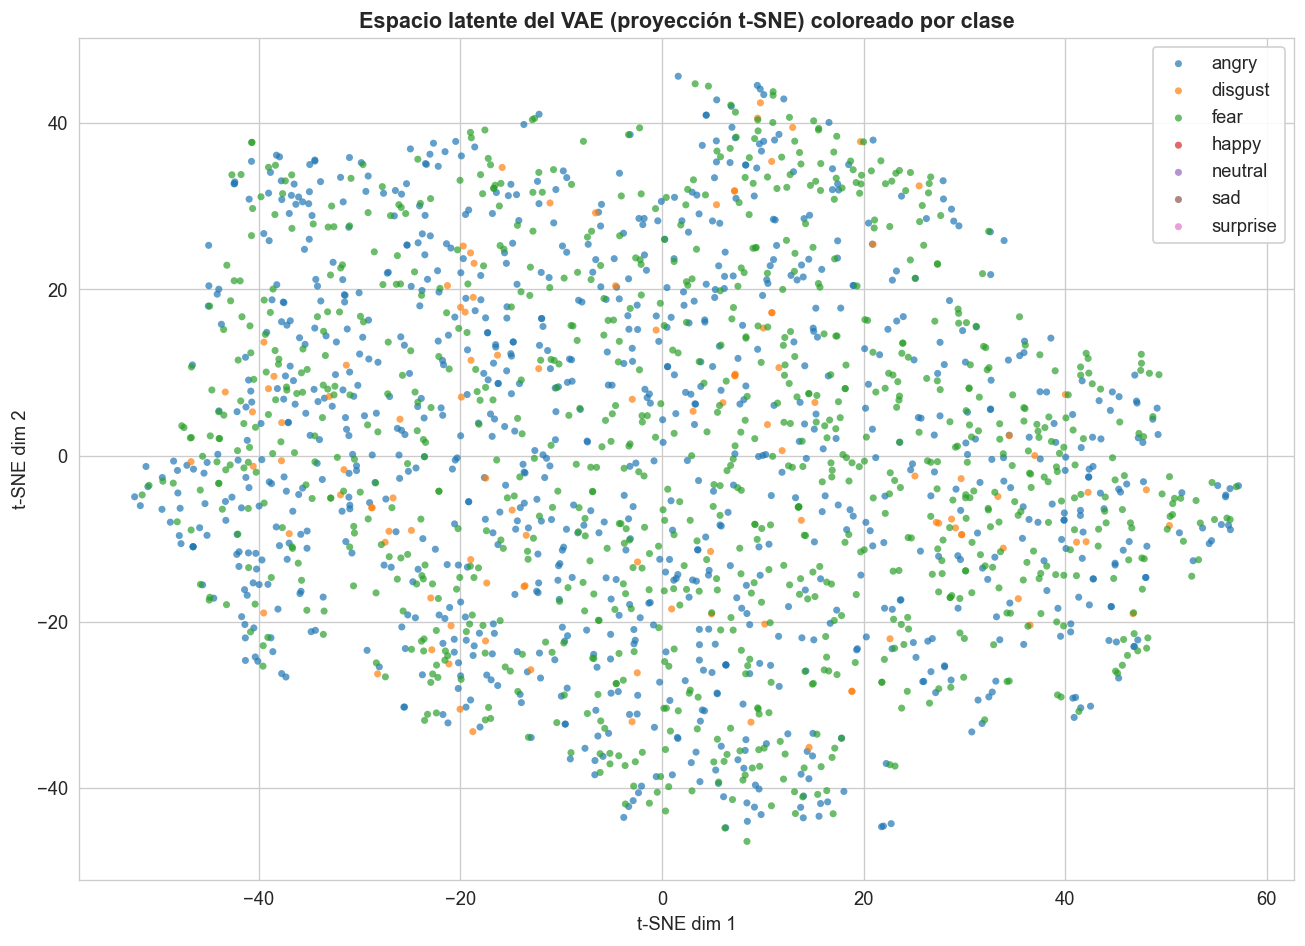
\includegraphics[width=\columnwidth]{../outputs/05_espacio_latente_tsne.png}
\caption{Proyección t-SNE de 2.000 vectores latentes del test set, coloreados por clase. Los clusters por clase \textbf{no} son claramente distinguibles — todas las clases se mezclan en una nube relativamente uniforme. Esto es esperable en un VAE no supervisado con KL bajo: el modelo aprende la \textit{distribución global} de rostros sin priorizar separabilidad por clase. La solución estructural es Conditional VAE (trabajo futuro).}
\label{fig:tsne}
\end{figure}

% =========================================================
%  6. DISCUSIÓN
% =========================================================
\section{Discusión y conclusiones}

El experimento valida empíricamente cuatro afirmaciones:

\begin{enumerate}[label=\arabic*.]
    \item \textbf{El truco de reparametrización funciona como teoría predice.} La pérdida ELBO desciende monotónicamente y el modelo aprende a reconstruir rostros reconocibles desde un espacio latente continuo regularizado.
    \item \textbf{El VAE estándar es numéricamente frágil.} Sin clips de \texttt{log\_var} y de la salida BCE, el modelo colapsa a NaN en pocas épocas. Sin calibración fina de $\beta$ y épocas, entra en posterior collapse. Esto no es un fracaso experimental — es una característica conocida de la familia VAE.
    \item \textbf{La borrosidad de las reconstrucciones es inherente al VAE con pérdida BCE.} Se promedia entre múltiples soluciones plausibles. Mitigable solo con cambios arquitectónicos profundos (VAE-GAN híbrido, modelos de difusión, transfer learning).
    \item \textbf{La interpolación es suave aunque sutil} en este modelo. Una interpolación más expresiva requiere mayor uso del espacio latente — un Conditional VAE separaría las clases en el latente y haría la interpolación más narrativa.
\end{enumerate}

\paragraph{Lecciones aplicadas al feedback acumulado.}
\begin{itemize}
    \item \textit{(Semana 1, ``más features'')}: el espacio latente del VAE es la materialización máxima del principio — features completamente aprendidas, cero ingeniería manual.
    \item \textit{(Semana 2, ``sin MaxPooling'')}: aplicado al 100\,\%. \texttt{Conv2D(stride=2)} y \texttt{Conv2DTranspose(stride=2)} preservan información que el pooling descartaría en imágenes 48$\times$48.
    \item \textit{(Semana 2, ``redes más grandes'')}: red de 1,6\,M parámetros (1,3$\times$ la CNN previa). La sección de trabajo futuro propone el siguiente salto natural (StyleGAN2 con $\sim$30\,M).
\end{itemize}

\paragraph{Conexión con LBD — Psico Platform.}

Tres aplicaciones directas del VAE entrenado:

\begin{enumerate}[label=(\alph*)]
    \item \textbf{Representación compacta del afecto facial} — 48 dimensiones frente a 2.304 píxeles. Input estandarizado para módulos de seguimiento longitudinal sin almacenar imágenes brutas (mejora privacidad).
    \item \textbf{Interpolación afectiva como recurso psicoeducativo} — herramienta visual para mostrar a usuarios que las emociones existen en un continuo, no en categorías discretas. Útil en psicoeducación sobre depresión y ansiedad.
    \item \textbf{Generación de datos sintéticos preservando privacidad} — análogo directo al caso HCAM (lectura EIG Campus L-IAA\_25\_001122). Permite entrenar modelos downstream sin exponer expedientes reales.
\end{enumerate}

% =========================================================
%  7. LIMITACIONES Y TRABAJO FUTURO
% =========================================================
\section{Limitaciones y trabajo futuro}

\textbf{Limitaciones reconocidas:}
\begin{itemize}
    \item Borrosidad de las reconstrucciones (intrínseco al VAE+BCE).
    \item Interpolación sutil — el modelo no separa fuertemente las clases en el latente.
    \item Resolución baja (48$\times$48 nativa).
    \item Sesgo del dataset (FER-2013 fue recolectado de Google Images en 2013).
\end{itemize}

\textbf{Trabajo futuro (en orden de prioridad):}

\begin{enumerate}[label=\arabic*.]
    \item \textbf{Conditional VAE (CVAE)} — condicionar la generación por clase $(z, \mathrm{clase}) \to x$. Solución directa al problema de interpolación sutil: permitiría ``genera una cara \texttt{happy}'' explícitamente y separaría las clases en el espacio latente.
    \item \textbf{Transfer learning con StyleGAN2-FFHQ} — usar el generador pre-entrenado en 70.000 rostros FFHQ de alta resolución como decoder. Entrenar solo un encoder hacia su espacio latente $\mathcal{W}^+$. Resuelve simultáneamente la borrosidad y la baja resolución. \textbf{Esta es la continuación más prometedora} y aborda directamente el feedback de Semana 2 sobre redes más grandes + fine-tuning.
    \item \textbf{$\beta$-VAE con $\beta < 0{,}5$} — para mejorar reconstrucción a costa de regularización. Útil si la prioridad es nitidez sobre generación coherente desde prior.
    \item \textbf{Aplicación clínica (caso HCAM)} — replicar el experimento del Hospital Carlos Andrade Marín: entrenar el VAE en imágenes médicas (radiografías, dermatología) para generar datasets sintéticos sin riesgo de exposición de pacientes.
\end{enumerate}

% =========================================================
%  Referencias
% =========================================================
\paragraph{Referencias.}
{\footnotesize
Kingma, D. P., \& Welling, M. (2014). \textit{Auto-Encoding Variational Bayes}, arXiv:1312.6114. (Paper original VAE.) ~$\bullet$~
Higgins, I. et al. (2017). \textit{$\beta$-VAE: Learning Basic Visual Concepts with a Constrained Variational Framework}, ICLR. ~$\bullet$~
Karras, T. et al. (2019). \textit{A Style-Based Generator Architecture for GANs (StyleGAN)}, CVPR. ~$\bullet$~
Goodfellow, I. et al. (2013). \textit{Challenges in Representation Learning}, ICML Workshop. (FER-2013) ~$\bullet$~
Barrett, L. F. et al. (2019). \textit{Emotional Expressions Reconsidered}, Psychological Science in the Public Interest 20(1):1--68. ~$\bullet$~
Lectura EIG Campus L-IAA\_25\_001122 — \textit{VAEs para generación de imágenes médicas sintéticas (HCAM)}.
}

\end{document}
